\subsection{Komposisjon}

\begin{frame}{Relasjonskomposisjon}
    Gitt to relasjoner $R \subseteq A \times B$ og $S \subseteq B \times C$, kan vi konstruere komposisjonen $S \circ R \subseteq A \times C$:\\
    $S \circ R := \{(a, c) | (a, b) \in R \land (b, c) \in S\}$
    \pause
    \begin{figure}%
        \centering
        \subfloat{{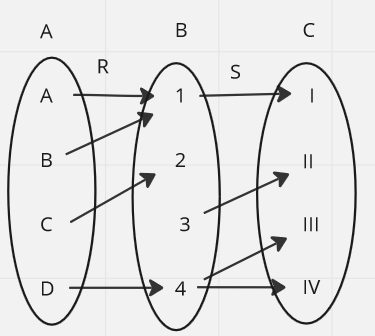
\includegraphics[width=3.3cm]{images/R, S.png} }}%
        \qquad
        \subfloat{{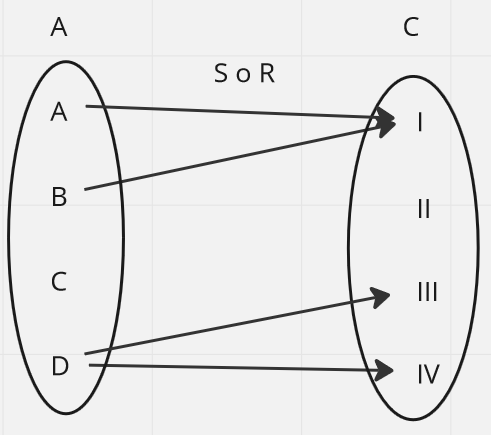
\includegraphics[width=3.3cm]{images/S o R.png} }}%
        \label{fig:ros}%
    \end{figure}
    \pause
    Obs! Som med funksjonskomposisjon er rekkefølgen er uintuitiv: R skjer før S. Dere kan lese det som $S$ 'på' $R$.
\end{frame}

\begin{frame}{Tavleoppgaver om relasjoner}
    Avgjør om følgende relasjoner er refleksive, symmetriske, anti-symmetriske, eller transitive. Er noen av dem ekvivalenserelasjoner?\\
    \begin{center}
    \begin{tabular}{ | m{15em} | m{1cm} | m{1cm} | m{1.5cm} | m{1cm} | m{1cm} | } 
      \hline
      Relasjon & Refl. & Symm. & A. Symm. & Trans. & Ekv.\\
      \hline
      $\{(a, b) | a, b \in \mathbb{N}, a < b\}$ \pause & \xmark & \xmark & \checkmark & \checkmark & \xmark \\
      \hline
      \pause
      $\{(a, b) | a, b \in \mathbb{N}, a \leq b\}$ \pause & \checkmark & \xmark & \checkmark & \checkmark & \xmark \\
      \hline
      \pause
      $B_{p, q}$ := Alle logiske uttrykk gitt av $p$ og $q$; $\{(a, b) | a, b \in B_{p, q}, a \equiv b\}$ \pause & \checkmark & \checkmark & \xmark & \checkmark & \checkmark\\
      \hline
      \pause
      $\emptyset$ \pause & \checkmark & \checkmark & \checkmark & \checkmark & \checkmark\\
      \hline
    \end{tabular}
    \end{center}
    \pause
    Merk at symmetri og antisymmetri ikke er helt det motsatte. En relasjon kan være begge deler (som $\emptyset$), og en relasjon kan være ingen av dem.
\end{frame}